\documentclass[aspectratio=169, 10pt]{beamer}

\usetheme{Madrid}
\usecolortheme{whale}

\usepackage{amsmath,amssymb,amsfonts}
\usepackage{booktabs}
\usepackage{graphicx}
\usepackage{tikz}
\usetikzlibrary{shapes.geometric, arrows.meta, positioning, calc, fit}
\usepackage{xcolor}

% Custom Colors matching ISMLL / academic styling
\definecolor{primaryblue}{RGB}{24, 76, 120}
\definecolor{accentorange}{RGB}{214, 90, 49}
\definecolor{darkgray}{RGB}{45, 52, 54}
\definecolor{lightgray}{RGB}{245, 246, 250}
\definecolor{successgreen}{RGB}{46, 117, 89}

\setbeamercolor{palette primary}{bg=primaryblue,fg=white}
\setbeamercolor{palette secondary}{bg=primaryblue!85,fg=white}
\setbeamercolor{palette tertiary}{bg=primaryblue!70,fg=white}
\setbeamercolor{structure}{fg=primaryblue}
\setbeamercolor{frametitle}{bg=primaryblue,fg=white}
\setbeamercolor{title}{bg=primaryblue,fg=white}

\setbeamertemplate{navigation symbols}{}
\setbeamertemplate{footline}[frame number]

\title[\textbf{Lightweight MTS: CycleNet-Pro \& SCPM}]{\textbf{Spectral Integrity, Modular Backbones, and Boundary Conditions in Lightweight Time Series Forecasting}}
\subtitle{Architecture Core: Diagnostics, Period Engine, and Spectral Patch Mixer}
\author[Chaturvedi et al.]{\textbf{Aaditya Chaturvedi} \and \textbf{Abdelhadi Hadj Sahraoui} \and \textbf{Philip Gentner} \and \textbf{Syed Natiq Hussain Shah} \\ \vspace{0.15cm}\small Supervisor: Jung Min Choi}
\institute[Univ.~Hildesheim]{Information Systems and Machine Learning Lab (ISMLL) \\ Institute for Computer Science, University of Hildesheim, Germany}
\date{October 2026}

\begin{document}

% =========================================================================
% TITLE SLIDE
% =========================================================================
\begin{frame}
  \titlepage
\end{frame}

% =========================================================================
% SLIDE 5: Normalized Diagnostics: FVU and LSD
% =========================================================================
\begin{frame}{4. Normalized Frequency Metrics: Scale-Free Diagnostics}
Because raw MSE is scale-dependent, we establish two physical diagnostic metrics:
\vspace{0.2cm}
\begin{columns}[T]
\column{0.50\textwidth}
\textbf{1. Fraction of Variance Unexplained ($FVU_{\text{band}}$):}
\begin{equation*}
    FVU_{\text{band}} = \frac{\sum_{k \in \mathcal{B}} w_k |E(k)|^2}{\sum_{k \in \mathcal{B}} w_k |Y(k) - \bar{Y}(k)|^2}
\end{equation*}
\begin{itemize}
    \item $FVU < 1.0$: Model learns genuine physical dynamics in that band.
    \item $FVU \approx 1.0$: Model performs no better than predicting a flat mean line.
    \item $FVU > 1.0$: Model actively hallucinates power and amplifies noise.
\end{itemize}

\column{0.50\textwidth}
\textbf{2. Log-Spectral Distance (LSD in dB):}
\begin{equation*}
    \text{LSD} = \sqrt{\frac{1}{M} \sum_{k=0}^{M-1} \left( 10 \log_{10} \frac{|\hat{Y}(k)|^2 + \epsilon}{|Y(k)|^2 + \epsilon} \right)^2}
\end{equation*}
\begin{itemize}
    \item Quantifies perceptual power spectral density (PSD) distortion across the full Nyquist range.
    \item Directly penalizes harmonic damping and spectral collapse.
\end{itemize}
\end{columns}
\end{frame}

% =========================================================================
% SLIDE 6: Automated CycleNet-Pro Overview
% =========================================================================
\begin{frame}{5. Proposed Solution: Automated CycleNet (CycleNet-Pro)}
\begin{center}
\textbf{Core Concept: Explicit Periodic Memory + Modular Residual Backbones}
\end{center}
\vspace{-0.2cm}
\begin{columns}[T]
\column{0.52\textwidth}
\begin{enumerate}
    \item \textbf{RevIN Instance Normalization}: Guards against global non-stationary distribution shifts.
    \item \textbf{Automated Period Discovery}: Dynamically extracts multi-period cycles via FFT + ACF (no hardcoded periods).
    \item \textbf{Recurrent Cyclic State Queues}: Maintains explicit learnable periodic parameters $\mathbf{Q}^{(k)}$.
    \item \textbf{Modular Residual Backbones}: De-cycles inputs and routes residuals through specialized backbones.
    \item \textbf{Residual Channel Mixing}: Selectively mixes inter-channel dependencies only when correlated.
\end{enumerate}

\column{0.48\textwidth}
\begin{figure}
\centering
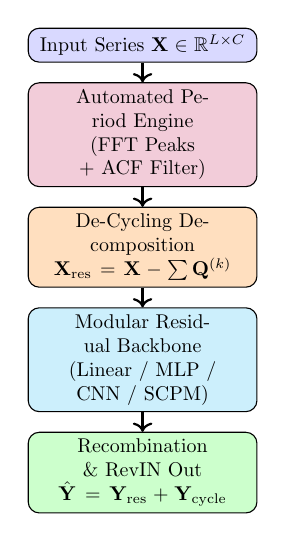
\begin{tikzpicture}[scale=0.72, every node/.style={transform shape}]
    \node[draw, rounded corners, fill=blue!15, text width=3.8cm, align=center] (inp) {Input Series $\mathbf{X} \in \mathbb{R}^{L \times C}$};
    \node[draw, rounded corners, fill=purple!20, below=0.35cm of inp, text width=3.8cm, align=center] (det) {Automated Period Engine\\(FFT Peaks + ACF Filter)};
    \node[draw, rounded corners, fill=orange!25, below=0.35cm of det, text width=3.8cm, align=center] (dec) {De-Cycling Decomposition\\$\mathbf{X}_{\text{res}} = \mathbf{X} - \sum \mathbf{Q}^{(k)}$};
    \node[draw, rounded corners, fill=cyan!20, below=0.35cm of dec, text width=3.8cm, align=center] (bb) {Modular Residual Backbone\\(Linear / MLP / CNN / SCPM)};
    \node[draw, rounded corners, fill=green!20, below=0.35cm of bb, text width=3.8cm, align=center] (rec) {Recombination \& RevIN Out\\$\hat{\mathbf{Y}} = \mathbf{Y}_{\text{res}} + \mathbf{Y}_{\text{cycle}}$};
    \draw[->, thick] (inp) -- (det);
    \draw[->, thick] (det) -- (dec);
    \draw[->, thick] (dec) -- (bb);
    \draw[->, thick] (bb) -- (rec);
\end{tikzpicture}
\end{figure}
\end{columns}
\end{frame}

% =========================================================================
% SLIDE 7: Automated Multi-Period Discovery Engine
% =========================================================================
\begin{frame}{6. Engine Stage 1: Automated Period Discovery (FFT + ACF)}
Prior models forced arbitrary hardcoded periodicities ($p=24$ or $p=96$). CycleNet-Pro discovers physical periods autonomously from training data:
\vspace{0.2cm}
\begin{columns}[T]
\column{0.33\textwidth}
\begin{block}{1. FFT Peak Ranking}
\begin{itemize}
    \item Compute power spectrum: $P(f) = |\text{rFFT}(\mathbf{x})|^2$.
    \item Extract candidate peaks via local extrema detection.
    \item Merge spectral leakage clusters within a 12\% relative distance.
\end{itemize}
\end{block}

\column{0.33\textwidth}
\begin{alertblock}{2. ACF Noise Filter}
\begin{itemize}
    \item Validate candidate periods using empirical Autocorrelation (ACF).
    \item 95\% white-noise confidence threshold:
    $$\text{Bound}_{\text{ACF}} = \frac{1.96}{\sqrt{N_{\text{train}}}}$$
    \item Eliminates spurious spectral peaks.
\end{itemize}
\end{alertblock}

\column{0.34\textwidth}
\begin{exampleblock}{3. Variance Decision}
\begin{itemize}
    \item Calculate marginal variance reduction of candidate cycles:
    $$\Delta \text{Var}(k) \ge 2.0\%$$
    \item Automatically accepts secondary/tertiary harmonics (e.g., intra-day + weekly cycles).
\end{itemize}
\end{exampleblock}
\end{columns}
\end{frame}

% =========================================================================
% SLIDE 8: Recurrent Memory Queues & De-Cycling
% =========================================================================
\begin{frame}{7. Engine Stage 2: Recurrent Periodic Queues \& De-Cycling}
\begin{columns}[T]
\column{0.55\textwidth}
\textbf{Explicit Recurrent State Formulation:}
\begin{itemize}
    \item For each discovered period $p_k \in \mathcal{P}$, maintain a learnable state matrix $\mathbf{Q}^{(k)} \in \mathbb{R}^{p_k \times C}$.
    \item Given global time index $\tau$, retrieve historical periodic pattern via circular phase indexing:
    \begin{equation*}
        \mathbf{C}^{(k)}_t = \mathbf{Q}^{(k)}_{(\tau + t) \pmod{p_k}}, \quad t \in [0, L-1]
    \end{equation*}
    \item \textbf{Residual De-Cycling:} Subtract periodic components from RevIN-normalized input:
    \begin{equation*}
        \mathbf{X}_{\text{res}} = \mathbf{X}_{\text{norm}} - \sum_{k=1}^K \mathbf{C}^{(k)}
    \end{equation*}
\end{itemize}

\column{0.45\textwidth}
\begin{block}{Why De-Cycling Works}
\begin{itemize}
    \item The residual $\mathbf{X}_{\text{res}}$ contains only non-periodic dynamics (secular trends, transient shocks, weather regime changes).
    \item The residual backbone does not waste capacity learning repetitive diurnal cycles.
    \item Periodic extrapolation to horizon $H$ is mathematically exact:
    $$\mathbf{Y}_{\text{cycle}, t} = \sum_{k=1}^K \mathbf{Q}^{(k)}_{(\tau + L + t) \pmod{p_k}}$$
\end{itemize}
\end{block}
\end{columns}
\end{frame}

% =========================================================================
% SLIDE 9: Modular Residual Backbones & SCPM Revision
% =========================================================================
\begin{frame}{8. Modular Residual Backbones: Specialization \& SCPM Revision}
CycleNet-Pro provides four modular, interchangeable residual backbones:
\vspace{0.15cm}
\begin{columns}[T]
\column{0.50\textwidth}
\begin{block}{1. Linear \& MLP Backbones}
\begin{itemize}
    \item \textbf{Linear}: Channel-independent $\mathbf{W} \in \mathbb{R}^{H \times L}$. Parameter-efficient baseline.
    \item \textbf{MLP}: 2-layer projection with hidden dimension 512 + GELU for non-linear temporal dynamics.
\end{itemize}
\end{block}
\begin{block}{2. 1D-CNN Backbone (Edge-Scale)}
\begin{itemize}
    \item Shared 1D-Conv across time and channels with linear length interpolation ($L \to H$).
    \item Slashes parameters by \textbf{97.7\%} (5.5k vs. 241k on ETT).
\end{itemize}
\end{block}

\column{0.50\textwidth}
\begin{exampleblock}{3. Revised SOR: SCPM Backbone}
\textbf{Spectral-Conditioned Patch Mixer (SCPM):}
\begin{itemize}
    \item \textbf{Intra-Patch Mixer}: Token MLP along time within each patch + feature MLP.
    \item \textbf{Inter-Patch Mixer}: Neighbor-aware gated MLP across local patch order + feature MLP.
    \item \textbf{FiLM Spectral Conditioning}: Reads orthonormal DCT-II log-energy subbands and dynamically modulates patch tokens:
    $$\mathbf{Z}_{\text{cond}} = \mathbf{Z} \odot (1 + \boldsymbol{\gamma}) + \boldsymbol{\beta}$$
    Zero-initialization ensures training starts strictly from identity.
\end{itemize}
\end{exampleblock}
\end{columns}
\end{frame}

% =========================================================================
% SLIDE 8b: Detailed Architecture of SORMixer (SCPM)
% =========================================================================
\begin{frame}{8b. SORMixer Architecture: Spectral-Conditioned Patch Mixer}
\centering
\vspace{-0.15cm}
\resizebox{!}{0.76\textheight}{%
    % SORMixer Presentation Architecture Diagram (Wide 16:9 Layout)
\providecolor{sorblue}{RGB}{24, 76, 120}
\providecolor{sororange}{RGB}{214, 90, 49}
\providecolor{sorgreen}{RGB}{46, 117, 89}
\providecolor{sordark}{RGB}{45, 52, 54}
\providecolor{sorlight}{RGB}{245, 246, 250}

\begin{tikzpicture}[
    >=stealth,
    font=\small,
    box/.style={draw, rounded corners=3pt, thick, align=center, inner sep=4.5pt, fill=white, font=\small},
    input/.style={box, fill=blue!10, draw=sorblue!80, text width=4.6cm},
    fold/.style={box, fill=cyan!12, draw=cyan!70!black, text width=4.6cm},
    patch/.style={box, fill=teal!12, draw=teal!70!black, text width=4.6cm},
    intra/.style={box, fill=orange!15, draw=sororange!80, text width=4.6cm},
    pool/.style={box, fill=teal!18, draw=teal!80!black, text width=4.6cm},
    film_node/.style={box, fill=purple!20, draw=purple!80!black, text width=4.6cm},
    inter/.style={box, fill=yellow!30!orange!18, draw=sororange!90, text width=4.6cm},
    head/.style={box, fill=cyan!18, draw=cyan!80!black, text width=4.6cm},
    output/.style={box, fill=sorgreen!20, draw=sorgreen!80!black, text width=4.6cm},
    spec/.style={box, fill=violet!12, draw=violet!70!black, text width=4.6cm},
    card/.style={draw=sordark!40, fill=sorlight, rounded corners=3pt, inner sep=5pt, font=\footnotesize, align=left}
]

% =========================================================================
% STAGE 1: Patch Formation & Intra-Patch Modeling (x = 0)
% =========================================================================
\node[font=\bfseries\normalsize, text=sorblue, anchor=center] (s1_title) at (0, 0.4) {1. Patch \& Intra-Mixer};

\node[input, below=0.22cm of s1_title] (in_res) {
    \textbf{Residual Input} $\mathbf{X}_{\text{res}} \in \mathbb{R}^{B \times L \times C}$\\
    \footnotesize De-cycled residual from CycleNet-Pro
};

\node[fold, below=0.22cm of in_res] (fold) {
    \textbf{Channel Fold} $\mathbf{X}_c$\\
    \footnotesize Reshape to $[B \cdot C, L]$ (Channel-Indep.)
};

\node[patch, below=0.22cm of fold] (patching) {
    \textbf{Unfold \& Point Embed}\\
    \footnotesize Patches: $[B \cdot C, N, P] \implies \mathbf{H}_0 \in [B \cdot C, N, P, D]$
};

\node[intra, below=0.22cm of patching] (intra) {
    \textbf{Intra-Patch Mixer}\\
    \footnotesize Time-MLP ($P \to 2P \to P$) + Feat-MLP ($D \to 2D \to D$)
};

\node[pool, below=0.22cm of intra] (pool) {
    \textbf{Patch Token Pooling}\\
    \footnotesize $\text{Linear}(P \cdot D \to D) \implies \mathbf{H} \in [B \cdot C, N, D]$
};

\draw[->, thick, color=sorblue] (in_res) -- (fold);
\draw[->, thick, color=teal!80!black] (fold) -- (patching);
\draw[->, thick, color=teal!80!black] (patching) -- (intra);
\draw[->, thick, color=sororange!90!black] (intra) -- (pool);

% =========================================================================
% STAGE 2: DCT-II Spectral Conditioning Branch (x = 5.5)
% =========================================================================
\node[font=\bfseries\normalsize, text=violet!85!black, anchor=center] (s2_title) at (5.5, 0.4) {2. Spectral FiLM Branch};

\node[spec, below=0.22cm of s2_title] (dct) {
    \textbf{Orthonormal DCT-II}\\
    \footnotesize $\mathbf{C}_{\text{dct}} = \mathbf{X}_c \mathbf{D}^T \in \mathbb{R}^{B \cdot C \times L}$ (Energy compaction)
};

\node[spec, below=0.22cm of dct] (spec_power) {
    \textbf{Log-Power Subbands}\\
    \footnotesize $\mathbf{S} = \log(1 + \mathbf{C}_{\text{dct}}^2) \to \text{Pool}(K=4) \implies \bar{\mathbf{s}} \in [B \cdot C, K]$
};

\node[spec, below=0.22cm of spec_power] (film_mlp) {
    \textbf{Zero-Init FiLM Generator}\\
    \footnotesize MLP: $K \to \text{hidden} \to 2D \implies (\boldsymbol{\gamma}, \boldsymbol{\beta}) = (\mathbf{0}, \mathbf{0})$
};

\node[film_node, below=0.28cm of film_mlp] (film) {
    \textbf{FiLM Spectral Modulation}\\
    $\mathbf{H}_{\text{cond}} = \mathbf{H} \odot (1 + \boldsymbol{\gamma}) + \boldsymbol{\beta}$\\
    \footnotesize \textit{Step 0: Identity Initialization ($\mathbf{H}_{\text{cond}} = \mathbf{H}$)}
};

% Connectors in Stage 2
\draw[->, thick, color=violet!80!black] (dct) -- (spec_power);
\draw[->, thick, color=violet!80!black] (spec_power) -- (film_mlp);
\draw[->, thick, color=purple!90!black] (film_mlp) -- (film)
    node[midway, right, font=\footnotesize] {$(\boldsymbol{\gamma}, \boldsymbol{\beta})$};

% =========================================================================
% STAGE 3: Inter-Patch Mixer & Forecasting Head (x = 11.0)
% =========================================================================
\node[font=\bfseries\normalsize, text=sororange!95!black, anchor=center] (s3_title) at (11.0, 0.4) {3. Inter-Patch \& Forecast};

\node[inter, below=0.22cm of s3_title] (inter) {
    \textbf{Neighbor-Gated Inter-Mixer}\\
    \footnotesize Context: $[\mathbf{h}_{i-1}, \mathbf{h}_i, \mathbf{h}_{i+1}] \in 3D \to \text{MLP}_{3D \to D}$\\
    \footnotesize Dynamic Gate $g_i \in [0, 1]$ + Feat-MLP
};

\node[head, below=0.22cm of inter] (head) {
    \textbf{Forecasting Head}\\
    \footnotesize $\text{Linear}(N \cdot D \to D) \to \text{GELU} \to \text{Linear}(D \to H)$
};

\node[output, below=0.22cm of head] (out_res) {
    \textbf{Residual Forecast} $\hat{\mathbf{Y}}_{\text{res}} \in \mathbb{R}^{B \times H \times C}$\\
    \footnotesize Unfold channels + Periodic forecast $\hat{\mathbf{Y}}_{\text{cycle}}$
};

\node[card, below=0.22cm of out_res, text width=4.6cm] (summary_card) {
    \textbf{Key SORMixer Specifications:}\\
    $\bullet$ \textbf{Params}: $\sim \mathbf{100\text{k}}$ ($10\times$ smaller than PatchTST)\\
    $\bullet$ \textbf{Complexity}: $\mathcal{O}(N)$ strictly linear in patches\\
    $\bullet$ \textbf{Channel}: Independent residual modeling\\
    $\bullet$ \textbf{Conditioning}: Orthonormal DCT-II FiLM
};

% Connectors between Stages
% Branch from Stage 1 Fold to Stage 2 DCT
\draw[->, thick, color=violet!80!black] (fold.east) -- ++(0.45, 0) node[midway, above, font=\footnotesize] {$\mathbf{X}_c$} |- (dct.west);

% Stream from Stage 1 Pool to Stage 2 FiLM
\draw[->, thick, color=teal!80!black] (pool.east) -- ++(0.45, 0) node[midway, above, font=\footnotesize] {$\mathbf{H}$} |- (film.west);

% Stream from Stage 2 FiLM to Stage 3 Inter-Patch (centered in corridor)
\draw[->, thick, color=purple!80!black] (film.east) -- ++(0.45, 0) node[midway, above, font=\footnotesize] {$\mathbf{H}_{\text{cond}}$} |- (inter.west);

\draw[->, thick, color=sororange!90!black] (inter) -- (head);
\draw[->, thick, color=sorgreen!80!black] (head) -- (out_res);

\end{tikzpicture}
%
}
\end{frame}

\end{document}
